% LaTeX Präsentationsvorlage (2013) der TU Graz, rev12, 2013/01/31
\documentclass{beamer}
\usepackage{pdfpages}
\usepackage{subfig}
\usepackage{tikz}
\definecolor{cFFFFFF}{rgb}{1.0, 1.0, 1.0}
\definecolor{cffffff}{rgb}{1.0, 1.0, 1.0}
\definecolor{c6E6E6E}{rgb}{0.2, 0.2, 0.2}
\definecolor{c030303}{rgb}{0.1, 0.1, 0.1}
\definecolor{c050505}{rgb}{0.3, 0.3, 0.3}
\tikzstyle{nome}=[draw, rectangle,anchor=center, minimum height=\altura,
  minimum width=9cm,fill=yellow!30,text width=8.8cm]

% \documentclass[aspectratio=169]{beamer}
\usetheme{tugraz2013}
% \usetheme[notes]{tugraz2013}
% \usetheme[minimal]{tugraz2013}

%% Titelblatt-Einstellungen
\title[Tagged Memory Security on RISC-V]{Tagged Memory Security on RISC-V}
\author{Philipp Jantscher}
\date{Graz, 18. December 2015}		% \today für heutiges Datum verwenden
%\date{\today}
\institute[IAIK]{IAIK}
\instituteurl{www.iaik.tugraz.at}
% \institutelogo{kurz.pdf}
% \additionallogo{institutslogo.pdf}

%%%%%%%%%%%%%%%%%%%%%%%%%%%%%%%%%%%%%%%%%%%%%%%%%%%%%%%%%%%%%%%%%%%%%%%%%%%%
\begin{document}
%%%%%%%%%%%%%%%%%%%%%%%%%%%%%%%%%%%%%%%%%%%%%%%%%%%%%%%%%%%%%%%%%%%%%%%%%%%%
\titleframe

\section{Outline}
\begin{frame}
	\frametitle{Outline}
	\begin{itemize}
		\item Motivation
    	\item Vulnerable buffer overflow attacks
    	\item RISC-V
    	\item Hardware and Toolchain
    	\item Tagged Memory
    	\item Untethered RISC-V
    	\item Tag Security Policies
    	\item Project Time-line
	\end{itemize}
\end{frame}


\section{Motivation}
\begin{frame}
	\frametitle{Motivation}
	Current Status
	\begin{itemize}
		\item Stack buffer overflow still a huge impact on security
    	\item Getting access to the computer by injection of code
    	\item No solution yet which protects this asset
	\end{itemize}
	Main Goals
	\begin{itemize}
		\item Implement strong Security policies using Tagged Memory
    	\item Efficient and Secure Solution
    	\item Effortless protection of  existing programs
    	\item Development on a open source processor 
	\end{itemize}
\end{frame}

\section{Buffer Overflows}
\begin{frame}
	\frametitle{Buffer Overflows}
	Stack and Heap often target of attacks due to programming errors (range checks)
	\begin{itemize}
		\item Leaks easy to fix,  also easy to oversee
		\item Attack can take control of machine
		\item Change of control flow
		\item Execution of arbitrary attacker code
	\end{itemize}
\end{frame}

\begin{frame}
	\frametitle{Modify Return Address}
	Unchecked length of input string - overwrites return address
	\begin{figure}[!h]
\begin{center}
%\includegraphics[width=9cm]{figures/reader_states.jpg}
\scalebox{0.4}{%
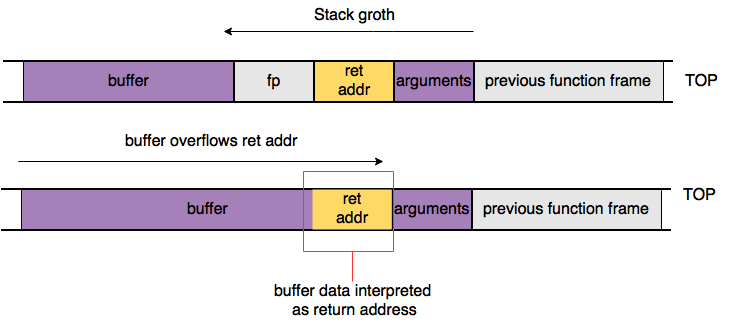
\includegraphics{figures/stack_return_overflow.png}
}
\end{center}
\end{figure}

\end{frame}

\begin{frame}
	\frametitle{Modify Pointer To Callback Function}
	Similar attack but operates also on heap ...
	\begin{itemize}
		\item callback function pointer somewhere in heap
		\item inject attack code by heap buffer overflow
		\item change the function pointer to point to attack code
	\end{itemize}
\end{frame}

\begin{frame}
	\frametitle{Modify Pointer To Callback Function}
	\begin{figure}[!h]
\begin{center}
%\includegraphics[width=9cm]{figures/reader_states.jpg}
\scalebox{0.4}{%
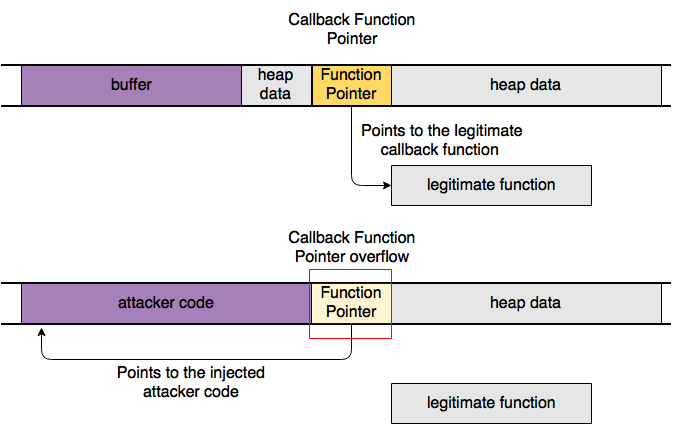
\includegraphics{figures/heap_callback_overflow-2.png}
}
\end{center}
\end{figure}

\end{frame}

\section{RISC-V}
\begin{frame}
	\frametitle{RISC-V}
	\begin{itemize}
		\item Open-Source processor, University of Berkley
		\item Optimized Instruction set for research topics
		\item Developed with Chisel
		\item PROCESSOR DATA
		\item Currently tethered to ARM-Processor (boot-strapping)
	\end{itemize}
\end{frame}

\begin{frame}
	\frametitle{RISC-V Processor Structure}
	ToDo: Other picture
	\begin{figure}[!h]
	\begin{center}
	%\includegraphics[width=9cm]{figures/reader_states.jpg}
		\scalebox{0.25}{%
		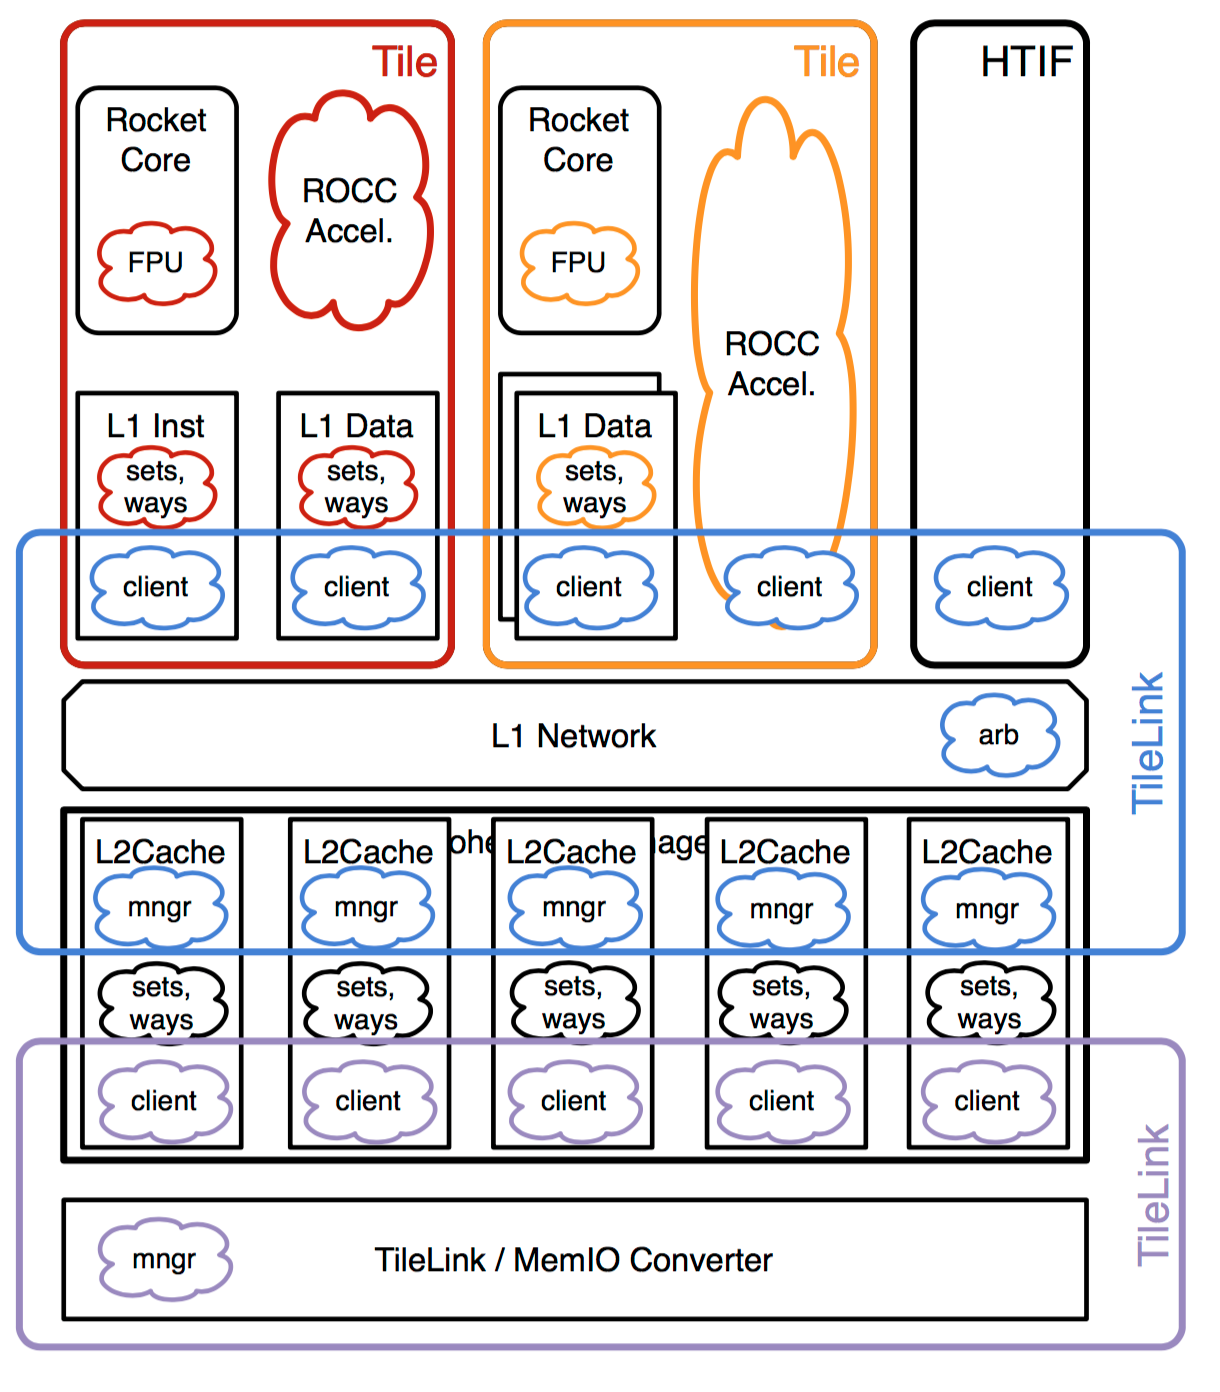
\includegraphics{figures/rocket.png}
	}
	\end{center}
	\end{figure}
\end{frame}

\begin{frame}
	\frametitle{The lowRISC project}
		Sub organisation 
		\begin{itemize}
		\item Goal to make a fully open SoC 
		\item Raspberry Pi for grown ups
		\item Community project to support hardware and application designers  
	\end{itemize}
\end{frame}

\section{Hardware and Toolchain}
\begin{frame}
	\frametitle{Hardware}
	Original designed for Zynq boards. This thesis will be done on Kintex-7
	\begin{itemize}
			\item Kintex 7 information
		\end{itemize}
\end{frame}

\begin{frame}
	\frametitle{Chisel}
	Developed by University of Berkley
	\begin{itemize}
		\item New high level hardware design language
		\item Based on Scala
		\item Full control over resulting RTL structures
		\item Powerful generator (e.g add and remove modules per define)
		\item Outputs: Cycle accurate C++ Emulator, Verilog
		\item Use Vectors, Maps, Objects within Scala
	\end{itemize}
\end{frame}

\begin{frame}
	\frametitle{Toolchain}
	Several software tools for development
	\begin{itemize}
		\item Fully adapted GNU Toolchain
		\item RISC-V bare-metal compiler
		\item RISC-V Linux compiler
		\item Simulation with C++ Emulator (Waveform output included)
		\item FPGA-implemenation using Verilog output and Xilinx Vivado
	\end{itemize}
\end{frame}

\section{Tagged Memory}
\begin{frame}
	\frametitle{Tagged Memory}
	Extension to RISC-V by lowRISC team.
	\begin{itemize}
		\item Ability to tag every 64 bits in memory with one or more tags
		\item So far only Framework (load and store tag)
		\item Additional Tag-Cache to improve performance
	\end{itemize}
	Changes to RISC-V
		\begin{itemize}
		\item Add L1 data cache support for tagged memory type
		\item TileLink size 512 to 544 bits to transfer data + tags
		\item Adding of Tag-Cache
	\end{itemize}
\end{frame}

\begin{frame}
	\frametitle{Tag Cache}
\begin{figure}[!h]
	\begin{center}
	%\includegraphics[width=9cm]{figures/reader_states.jpg}
		\scalebox{0.2}{%
		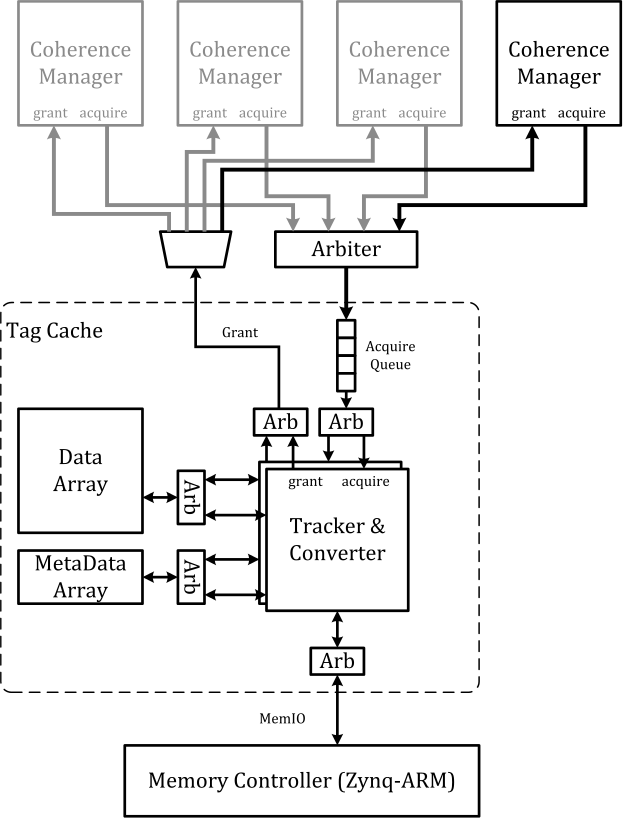
\includegraphics{figures/tag_cache.png}
	}
	\end{center}
	\end{figure}
\end{frame}

\section{Untethered RISC-V}
\begin{frame}
	\frametitle{Current RISC-V}
	Currently RISC-V is thehered to ARM-Processing System
	\begin{itemize}
	\item HostIO: AXI Lite interface for Input/Output handled by ARM
	\item MemIO: AXI HP for DDR3 Memory access through ARM
	\item Boot strapping
	\item RISC-V Frontend Server handles console in/out
	\end{itemize}
\end{frame}

\begin{frame}
	\frametitle{Current Structure}
	\begin{figure}[!h]
		\begin{center}
	%\includegraphics[width=9cm]{figures/reader_states.jpg}
		\scalebox{0.38}{%
		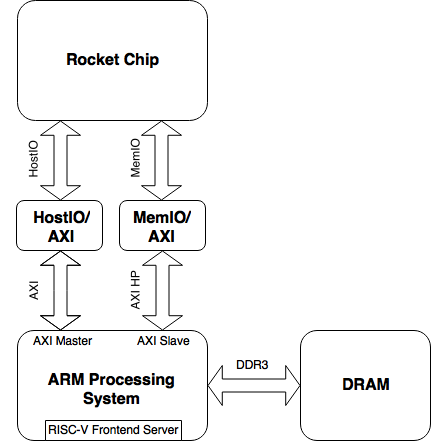
\includegraphics{figures/rocket_fpga_setup.png}
	}
	\end{center}
	\end{figure}
\end{frame}

\begin{frame}
	\frametitle{Changes for Untethering}
	lowRISC team implemented untethered version on Kintex-7 board (upcoming release)
	\begin{itemize}
	\item MemIO exchanged with NASTI-Bus (Berkley AXI-4 implementation)
	\item HostIO for debug purposes
	\item Adding IO devices like UART and SPI
	\item IO interface is NASTI-Lite
	\item Implementation of IO memory map
	\item internal and external Bus width reduced to 128 bit (4 bursts for one cache line)
	\item Tagged Memory not ported yet.
	\end{itemize}
\end{frame}

\begin{frame}
	\frametitle{Untethered Structure}
	\begin{figure}[!h]
	\begin{center}
	%\includegraphics[width=9cm]{figures/reader_states.jpg}
		\scalebox{0.32}{%
		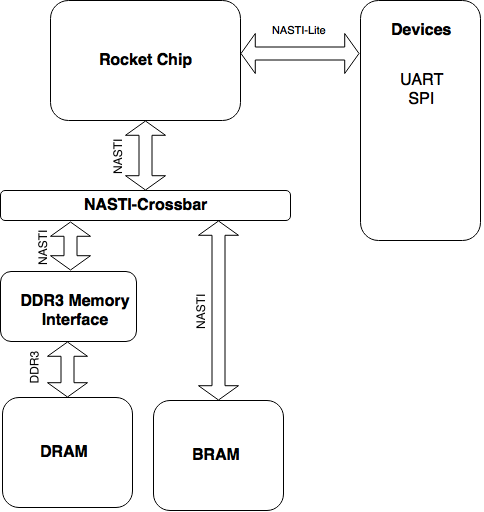
\includegraphics{figures/rocket_soc_setup.png}
	}
	\end{center}
	\end{figure}
\end{frame}

\section{Tag Security Policies}

\begin{frame}
	\frametitle{Tag Security Policies}
   Idea: Secure return address and function pointers from attackers
   \begin{itemize}
	   \item Only minor to no change to existing Programs (Linux context switch)
 	  \item Use of 2 tag bits (Bit 1: DATA/INVALID, Bit 2: RETURN)
 	  \item Implementation in untethered version
 	  \item Tag Control Unit that checks tags and causes traps/reset   
 	  \item No changes to compiler aimed for these policies
   \end{itemize}
\end{frame}

\begin{frame}
	\frametitle{Return Address Protection}
	\begin{enumerate}
	\item Function Call: JAL stores return address to stack. Tags memory as RET
	\item Attacker overwrites return address. RET tag cleared.
	\item JAL-R tries to jump to address in RA register without tag (trap performed).
	\end{enumerate}
	\begin{figure}[!h]
		\begin{center}
	%\includegraphics[width=9cm]{figures/reader_states.jpg}
		\scalebox{0.35}{%
		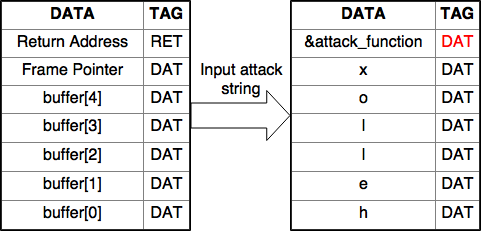
\includegraphics{figures/rat_address_tag.png}
	}
	\end{center}
	\end{figure}
\end{frame}

\begin{frame}
	\frametitle{Function Pointer Protection}
	\begin{enumerate}
	\item Data and function pointers tagged as DATA
	\item Attacker injects code and overwrites function pointer. (IO input causes INV tag)
	\item JAL-R tries to jump to address with INV tag(trap performed).
	\end{enumerate}
	\begin{figure}[!h]
		\begin{center}
	%\includegraphics[width=9cm]{figures/reader_states.jpg}
		\scalebox{0.35}{%
		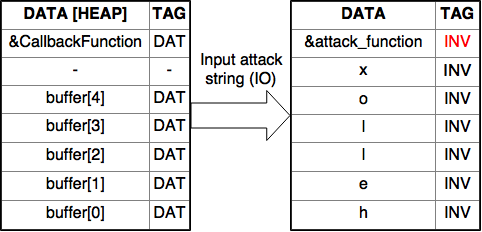
\includegraphics{figures/callback_fp_tag.png}
	}
	\end{center}
	\end{figure}
\end{frame}

\section{Project Time-line}

\begin{frame}
	\frametitle{Project Time-line}
   \begin{itemize}
   	  \item Preparation and lowRISC tutorial. 1.12.2015, 180h [Done]
	   \item Implementation of Tagged Memory. 31.01.2015, 150h
	   \item Tag Security Policies. 31.04.2015, 200h
		\item Documentation. 31.05.2015, 200h
   \end{itemize}
\end{frame}




%%%%%%%%%%%%%%%%%%%%%%%%%%%%%%%%%%%%%%%%%%%%%%%%%%%%%%%%%%%%%%%%%%%%%%%%%%%%
\end{document}
%%%%%%%%%%%%%%%%%%%%%%%%%%%%%%%%%%%%%%%%%%%%%%%%%%%%%%%%%%%%%%%%%%%%%%%%%%%%

%% EOF
